% This is samplepaper.tex, a sample chapter demonstrating the
% LLNCS macro package for Springer Computer Science proceedings;
% Version 2.20 of 2017/10/04
%
\documentclass[runningheads]{llncs}
%
\usepackage{graphicx}
% Used for displaying a sample figure. If possible, figure files should
% be included in EPS format.
%
% If you use the hyperref package, please uncomment the following line
% to display URLs in blue roman font according to Springer's eBook style:
% \renewcommand\UrlFont{\color{blue}\rmfamily}
% For correct quotation marks (command \enquote)
\usepackage{csquotes}

\begin{document}
%
\title{Interpretable Machine Learning -- A Short History, State of the Art and Challenges\thanks{This project is funded by the Bavarian State Ministry of Science and the Arts and coordinated by the Bavarian Research Institute for Digital Transformation (bidt) and supported by the German Federal Ministry of Education and Research (BMBF) under Grant No. 01IS18036A.
The authors of this work take full responsibilities for its content.
}}
%
%\titlerunning{Abbreviated paper title}
% If the paper title is too long for the running head, you can set
% an abbreviated paper title here
%
\author{Christoph Molnar\inst{1}\orcidID{0000-0003-2331-868X}}
%\and
%Second Author\inst{2,3}\orcidID{1111-2222-3333-4444} \and
%Third Author\inst{3}\orcidID{2222--3333-4444-5555}}
%
\authorrunning{Molnar}
% First names are abbreviated in the running head.
% If there are more than two authors, 'et al.' is used.
%
\institute{LMU Munich, Ludwigstr. 33, 80539 Munich, Germany
\email{christoph.molnar@gmail.com}\\
\url{https://www.slds.stat.uni-muenchen.de/people/molnar/}}
%
\maketitle              % typeset the header of the contribution
%
\begin{abstract}
  I present a very short history of the field of interpretable machine learning (IML), give an overview of popular interpretation methods and discuss challenges when interpreting machine learning models.

\keywords{Interpretable Machine Learning \and Explainable AI}
\end{abstract}
%
%
Interpretability is often a deciding factor when machine learning (ML) is used in a product, a decision process or in research.
With interpretable machine learning (IML) \footnote{We will be using Interpretable Machine Learning and Explainable AI exchangably} the user can find out problems, extract insights and justify decisions.
%I want to give three very common use cases:
%\paragraph{For science:} In applied sciences, data is often modeled with ML nowadays, where before statistical modeling approach would have been used.
%The goal of science is not only to predict the world well, but also to generate further insights.
%Examples are species distribution models in ecology which aim to explain why certain species can be found on certain areas based on e.g. the local climate.
%Here, interpretability of the prediction model is needed to understand why a species, e.g., has a high probability to occur in a specific reason.

TODO: Mention sensitivity analysis


\paragraph{A Very Short History of IML.}
Learning interpretable prediction models from data is not new, but has been the focus of statistical learning and rule-based ML for a long time.
Statistics has a long tradition of learning interpretable prediction  models from data, starting in 1800 \cite{stigler1986history} with works on least squares by Legendre 1805, \cite{legendre1805nouvelles}, Gauss in 1809 \cite{gauss1809theoria} and Quetelet in 1827 \cite{quetelet1827recherches}.
Another methodological pillow are rule-based machine learning approaches, which includes models such as decision rules and decision trees.
Many extensions exists, such as non-linear transformations for the case that the target follows a different distribtuion (GLMs, logistic regression).
The beauty of linear models is that they are additive, meaning that the influences of each feature on the target can be added together to give the full effect.
  This took off in the 80s with decision tree approaches such as CART and ID3 and rule learners like AQ \cite{furnkranz2012foundations} but reaches back to first research in the 1960s \cite{hajek1966guha}.
Both research on linear regression models and its extensions and rule-based ML remain important and busy research areas to this day and are even blending together (e.g. model-based trees \cite{zeileis2008model}).
As a next stepping stone to the field of IML are random forests, an early approach to explain more complex machine learning models.
I argue that one of the success factors of the random forest as a prediction model was (and is) the built-in feature importance measure.
The high citation counts (>60000 citation on Google Scholar as of September 2020) of the original paper \cite{breiman2001random}, but also suggestions for how to improve the random forest feature importance (\cite{strobl2008conditional,strobl2007bias,hapfelmeier2014new,ishwaran2007variable}) are evidence for this.

In 2010s then came the deep learning hype.
And a few years after that, the IML field really took off in around 2015, judging on usage of the search terms "Interpretable Machine Learning" and "Explainable AI" on Google (Figure \ref{fig:count} right)and papers published with these terms (Figure \ref{fig:count} left).
\begin{figure}
  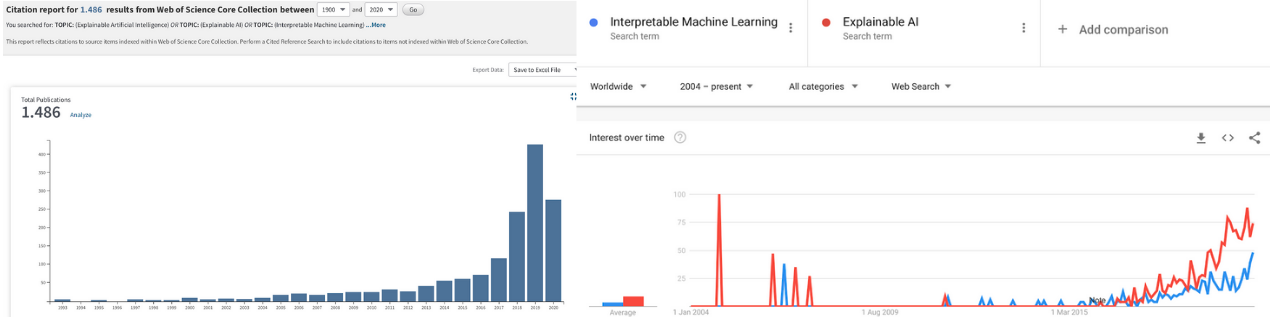
\includegraphics[width=\textwidth]{citation-search.png}
  \caption{Left, Right}
  \label{fig:count}
\end{figure}
Could it be that only the terms have changed, but the field has always been there and the same?
I would still argue that the field has reached a new form, as evidenced by new keywords "Interpretable Machine Learning" and "Explainable Artificial Intelligence", but also by bringing in new ideas from other fields, pulling many unconnected research fields together and an additional focus on model-agnostic ML interpretation methods.
I would say no, since a lot of commonly used methods, especially model-agnostic ones and the ones for deep neural network also came about this time.
These figures look like there has not been much research on explaining prediction models before, which would be a wrong conclusion, since developments happened under different names and in different fields.
What has changed is that Interpretable Machine Learning or Explainable Artificial Intelligence has become a field that now ties all these topics together.


\paragraph{Today} we have reached a first state of maturity where some methods were established, implemented in software and used by practitioners and applied researchers.
There is a lot of open source software that implement various techniques (\cite{iml,biecek2018dalex,pedregosa2011scikit,klaise2020alibi,nori2019interpretml}, ...).
Big tech companies offer software \cite{exler2019if,arya2020ai,hall2017machine}...
Regulation such as GDPR has spurred a discussion around further needs of interpretability.
Many startup are now focused on explainable / interpretable ML (TODO: Find good source).


\section{Methods:}

In this section I want to very broadly talk about methods that we have to explain models.
However we interpret a model, the interpretation is always projected back to the features themselves or some abstract transformation of them.
Often the distinction is made between model-specific (works only for one type of model) and model-agnostic (works for all models) interpretation methods.
I want to distinguish between introspection and sensitivity analysis.
An interpretation method that works by introspection assigns semantic meaning to \textit{(learned) model parameters and structures} while sensitivity analysis \textit{probes the model and describes its behavior}.
Introspection is necessarily model-specific.
Sensitivity analysis is mostly model-agnostic, but can also be done by leveraging model-specific knowledge such as gradient-based methods. \footnote{An example are the various heatmap-like explanation for CNNs for image classification \cite{sundararajan2017axiomatic,lundberg2017unified,montavon2017explaining,simonyan2013deep,shrikumar2016not} which study the sensitivity of the prediction to the input pixels. Technically this is done by backpropagation and therefore model-specific. Model-agnostic versions \cite{ribeiro2016should,lundberg2017unified,zeiler2014visualizing} exist.}
The other useful category is local vs. global explanations.
Local means that the method explains individual predictions, and global means it explains the average model behavior.
For inherently interpretable models, global and local explanations are often the same: In linear models, the coefficients both how the model behaves globally, but also is used for individuals instances.

\paragraph{Inherently interpretable models} are models where we can interpret its learned structure and parameters.
As a rule of thumb for when we do an introspection is that we are not probing the model with various (manipulated data points).
In this category, I see all linear regression models of the form $Y = \beta_0 + \beta_1 x_1 + \ldots + \beta_p x_p$, where the weights $\beta$ are learned parameters of the model.
Through the models structure (weighted sum of features) we can interpret the weights as the effect that a feature has on the prediction.
Similarly, decision trees and other rule-based ML models have a learned structure which we can interpret as how the model makes a prediction.
For example, an individual prediction can be traced through a decision tree and we retrieve an explanation of the form "If feature $x_1$ larger than two and feature $x_4$ in category A, then prediction is 10".
However, the more complex these structures get (e.g., a linear model with hundreds of features and complex interaction terms or very deep decision trees), the more difficult it becomes to see this as interpretable.
Surprisingly, we can also try assign meaning to structures of more complex models such as individual neurons or layers in a convolutional neural network.
This leads to the famous results where we find out that CNNs learn edge detectors at the lowest levels and increasingly abstract concepts at higher layers.
Another example is the random forest minimal depth distribution:\cite{randomForestExplainer}
The distribution of minimal depth shows for a feature for all the trees in the forest at which depth it occurs, with the notation that it the feature is more important if it appears early in the tree, it is more important.
This is again an example how we analyze the structure of a model to get an understanding of how it makes decisions, but the model is more complex (hundreds of decision trees) so there is more work to interpreting its learned structure.
The random forest is also a useful example for another measure, the feature importance, for which various measures exist, such as decrease in accuracy and decrease in Gini impurity.
By using our distinction of introspection and sensitivity analysis Gini impurity would fall into the former while mean decrease accuracy falls into the latter.
Gini importance collects for each feature and tree how the split decreased the Gini impurity.
It does not rely on making predictions, but only on internal statistics.
For mean decrease accuracy, we probe the random forest with perturbed data, i.e., we shuffle a feature and see how the prediction changes.
It's a model-specific methods since we do this tree-wise and use the out-of-bag sample of the tree, so this procedure is cleverly adapted to the random forest.
Model-agnostic versions of this permutation feature importance exists \cite{fisher2019all}.

\paragraph{Sensitivity-analysis-like (model-agnostic) interpretation methods} often treats the model as a black-box (but not always).
Here I also want to distinguish between local and global explanations.

\paragraph{Local explanations} explain how individual predictions are derived.
Here we have a great variety of methods, with very different methodological motivations.
Popular methods are LIME, Shapley Values and Counterfactual Explanations.
I want to highlight especially their very different approaches to the problem of local explanations.
Counterfactual explanations are what-if scenarios.
How does an instance have to change to get another (desired) prediction or classification.
They build on a rich tradition in philosophy and also thrive in what the social sciences discovered:
Good explanations are contrastive and focus on a few reasons.
A very different approach originates from collaborative game theory: The Shapley Values.
How do you fairly share some payout from a game among the players?
The Shapley values \cite{shapley1953value} provide an answer for this question, by trying out all constellations of players and averaging the additional payout a player would add to the total payout when the player is added to a team.
The same idea can be applied to ML: The predicted value is the payout, the player is a certain feature value.Many variations, extensions and more efficient implementations for specific ML models exist \cite{vstrumbelj2014explaining,lundberg2017unified,lundberg2018consistent}.
The third mention here are local interpretable model-agnostic explanations, short LIME \cite{ribeiro2016should}
LIME is a surrogate model, i.e., the procedure approximates the original ML model with a simpler interpretable model.
LIME does so locally, meaning only in some neighborhood around the data point that we want to explain.

\paragraph{Surrogate Models} are an interesting and huge class of explanation method \cite{puri2017magix,molnar2019,ming2018rulematrix}.
This approach is very common in sensitivity analysis where we have emulation? models.
Many methods -- a confusing amount, really -- are nothing but simple models that approximate the behavior of the (complex) model to be explained.
Surrogate models combine the two strategies:
First, approximate the predictions of the ML model with an interpretable model, such as a decision tree.
This is a kind of sensitivity-like approach, where we see the original model as a black box and artificially probe the ML model and derive information from the behavior.
Then we interpret the interpretable model, which now acts as a surrogate to the more complex ML model.
There are also methods for extracting, e.g., decision rules from specific models based on their internal components such as weights \cite{andrews1995survey,augasta2012rule}, which would be more the introspection approach.

\paragraph{Global, model-agnostic explanation methods} are also very popular.
Here we have have feature importance, which rank features based on how relevant they were for the prediction and the feature effect, which expresses how a change in that feature changes the predicted outcome on average.
Permutation Feature Importance \cite{fisher2019all}, which is based on permuting features is popular importance measure, originally suggested for random forests \cite{breiman2001random}, now available as model-agnostic version.
Alternatives are variance based measures, see \cite{wei2015variable} for an overview of all the ways to measure importance.
For feature effects we have Partial Dependence Plots \cite{friedman2001greedy}, Individual Conditional Expectation Plots \cite{goldstein2015peeking} and Accumulated Local Effect  (ALE)  Plots \cite{apley2016visualizing}.


\section{Challenges}

This is an incomplete list of some of the challenges of IML, mostly based on \cite{molnar2020pitfalls}.

\paragraph{Feature dependence:} When two features share information (e.g., BMI and weight) separating their effects and importances is difficult.
Some IML methods (e.g.LIME, permutation feature importance or Shapley values) simply \enquote{ignore} such dependence, which results in extrapolation, i.e., for the interpretation new, unrealistic data points are created (e.g., low weight but high BMI).
Interpretations based on extrapolation into areas where the model never saw data can be very misleading \cite{hooker2019please}.
There have been attempts to \enquote{fix} IML methods by creating only realistic data points (using the conditional instead of the marginal distribution).
These conditional IML methods fix the extrapolation problem, but they also entangle the interpretations of a feature's effect and importance with all other features it depends on.
In the case of Shapley values the conditional variant even breaks the interpretation \cite{sundararajan2019many,janzing2019feature}.

\paragraph{Uncertainty quantification} is a typical part of statistical modeling and becomes visible as error bars, confidence intervals, test statistics and p-values.
Uncertainty quantification helps to separate signal from noise.
Many IML methods only return the point estimates, but don't quantify the uncertainty.
This reaches across most methods: rule-based ML , feature effect plots, feature importance, ...
There is research about uncertainty quantification of model interpretations, e.g., feature importance \cite{watson2019testing,fisher2019all}, layer-wise relevance propagation \cite{fabi2020feature} and Shapley values \cite{williamson2020efficient}.
However, it is not implemented as default in most IML software.
Also we need a more united view on the topic, and specify which uncertainty is quantified (model bias, model variance, IML estimation error, ...) and to what end.
The statistics community is very deep into statistical inference and IML can learn a lot.
Here we have to dig deeper into the statistics literature which can be our guide.

\paragraph{Statistical inference:}
When uncertainty quantification is combined with assumptions about the data generating process, we can draw conclusions about the real world.
But for that we have to better understand the properties and assumptions of the various IML methods.
For example, methods such as partial dependence plots require that features are independent.
To enable statistical inference, there are at least two challenges to overcome: 1) define the assumptions needed that allow a model (and an IML method) to be interpreted as the \enquote{true} model and 2) tools and procedures to check these assumptions.

\paragraph{Causal interpretation}
Ideally, a model relies on the true causes to make a prediction.
Then we could also interpret it causally, making statements about the underlying phenomenon, which is the focus of ML in research, but also makes models robust against adversarial attacks, but also makes the model more usefule when used as a basis for decision making.
Unfortunately, predictive performance and causality can be conflicting goals.
For example, today's weather directly causes tomorrow's weather, but we might only have access to feature \enquote{wet ground}.
Using \enquote{wet ground} in the prediction model for \enquote{tomorrow's weather} is useful as it has information about \enquote{today's weather}, but we are not allowed to interpret it causally, because the confounder \enquote{today's weather} is missing.
Further research is needed to understand when we are allowed to make causal interpretations of an ML model.

\paragraph{Lack of definition} is a common critique of the field \cite{lipton2018mythos,doshi2017towards}.
Without a definition of "interpretability", how can we decide if a new method is better at explanation an ML method?
To evaluate the \textbf{predictive performance} of an ML model, we simply compute the prediction error on test data given the groundtruth label.
To evaluate the \textbf{interpretability} of that same ML model is not as easy.
We do not know what the groundtruth explanation looks like and have no straightforward mean to quantify how interpretable a model is or how correct an explanation is.
Instead of having one groundtruth explanation, various \textbf{quantifiable aspects of interpretability} are emerging.\cite{poursabzi2018manipulating,philipp2018measuring,molnar2019quantifying,hauenstein2018computing,zhou2018measuring,akaike1998information,schwarz1978estimating,poursabzi2018manipulating,dhurandhar2017tip,friedler2019assessing}
Sparsity of the explanation (or the model itself), interaction strength of features within the ML model and
It seems like we are on our way to have many definitions of \textit{various aspects} of interpretability such as sparsity, interaction strength and a user's ability to run a model on a given input (simulatability) are examples of such aspects.
The challenge ahead remains to establish a best practice on how to evaluate interpretation methods and the explanations they produce.

We have focused mostly on the methodological, mathematical challenges in a rather static setting, where you are given a machine learning model and data.
\paragraph{Many more} challenges lie ahead to improve interpretability of machine learning.
What is the best way to explain a machine learning model for people with a specific background and how do we present the explanations?
How are people affected by explanations, how are explanations maybe misused (CITE fairwashing by HIma)?
This is also a rather static view point in the sense that we can do a lot if we allow a more interactive way of modeling and "having a conversation" between a person and the model or even the modeling process.
How do we present multiple maybe conflicting explanations, e.g., when you generate multiple counterfactual explanations?

\section{Discussion}

Interpretable Machine Learning is a young field, but has deeper roots in Statistics and Computer Science and also draws from other fields such as the social sciences.
There has been Cambrian explosion of methods since 2015, including model-agnostic interpretation methods and many specialised methods for, e.g., deep neural networks.
Many of these methods have found their way into open source software and products of startups and tech companies.
Interpretable Machine Learning is used in science, company products and processes.
While we have reached a first maturity, there a still some challenges ahead, such as feature dependence, causality and inference.
Many IML methods are imported from other fields, so thinking outside the box (pun intended) might help in the challenges ahead.
We believe that the field has to both reach out horizontally -- to other domains -- and vertically -- draw from the rich research in statistics and computer science.


%
% ---- Bibliography ----
%
% BibTeX users should specify bibliography style 'splncs04'.
% References will then be sorted and formatted in the correct style.
%
% \bibliography{mybibliography}
%

\vskip 0.2in
\bibliographystyle{splncs04}
\bibliography{Bib}

\end{document}
